\documentclass[a4paper,12pt]{article}
\usepackage[utf8]{inputenc} 
\usepackage[T1]{fontenc} 
\usepackage[spanish]{babel} 
\usepackage{lmodern}             
\usepackage[hidelinks]{hyperref} 
\usepackage{graphicx}  
\usepackage{float}
\usepackage{bytefield}
\usepackage{geometry}
\usepackage{placeins}
\usepackage{fancyhdr} 

\geometry{left=2.5cm, right=2.5cm, top=3cm, bottom=3cm}
% Configuración de encabezado y pie de página
\pagestyle{fancy}

\title{\textbf{Configure IPv6 over IPv4 GRE Tunnel}}

\author{
    \begin{tabular}{c}
        Martin Moloeznik y Nicolas Paz Reyes \\
        \texttt{martinmoloeznik@gmail.com, rubenpaz2105@gmail.com} \\
        \href{https://github.com/N1C0-P4Z/IPv6-over-IPv4-GRE-Tunnels}{Repositorio en GitHub}
    \end{tabular}
}

\date{Abril 02, 2025}

\begin{document}

\maketitle

\section{Introduccion}
La configuración de túneles GRE (Generic Routing Encapsulation) permite encapsular paquetes IPv6 dentro de paquetes IPv4, facilitando la comunicación entre redes IPv6 a través de infraestructuras IPv4 existentes. Esta técnica es especialmente útil durante la transición de IPv4 a IPv6, ya que evita la necesidad de actualizar toda la infraestructura de red.
\section{Configuración del router en IPv6}
\begin{figure}[h]
    \centering
    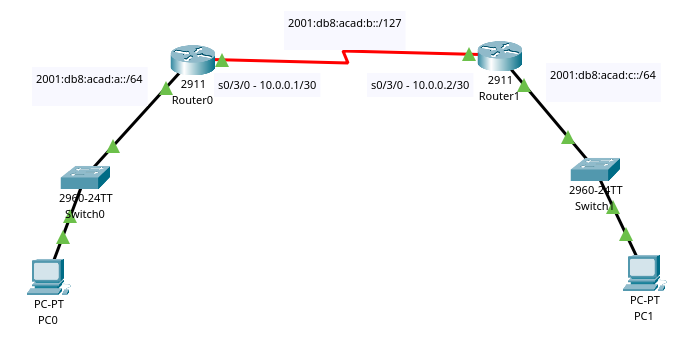
\includegraphics[width=1\textwidth]{imagenes/lab1.png}
    \caption{Escenario Modelo}
  \end{figure}
\FloatBarrier

Creamos un escenario usando 2 routers 2911(colocando en cada uno un module HWIC-2T), 2 switches 2911 y 2 PCs como se observa en la figura 1. Configuraremos la red de la PC0 y la PC1 con IPv6 y la red entre ambos routers con IPv4. El objetivo es lograr hacer que ambas PCs se comuniquen usando IPv6 a través de IPv4.\\
\subsection{Comandos de configuración}

Como primer paso configuramos la IPv6 y el default gateway de ambas PCs, como se ve a continuación:\\

\begin{table}[h]
    \centering
    \begin{tabular}{|c|c|c|}
        \hline
        \textbf{Dispositivo} & \textbf{Dirección IPv6} & \textbf{Gateway Predeterminado} \\
        \hline
        PC0 & 2001:db8:acad:a::1/64 & 2001:db8:acad:a:: \\
        \hline
        PC1 & 2001:db8:acad:c::1/64 & 2001:db8:acad:c:: \\
        \hline
    \end{tabular}
    \caption{Configuración de direcciones IPv6 de PC0 y PC1}
    \label{tab:ipv6_config}
\end{table}

Ahora antes de configurar los routers, ejecutamos en ambos switches:\\
\noindent\\
Switch(config)\#no spanning-tree vlan 1\\
Switch(config)\#no cdp run\\\\
Con el objetivo de evitar usar los protocolos CDP y STP que podrian causar problemas y son innecesarios para el objetivo de este escenario.\\
\subsection{Configuracion IPv6 de ambos routers}
Activamos el ruteo IPv6 en ambos \textbf{Routers} en el \textit{modo} global config con:\\

R0(config)\#ipv6 unicast-routing\\

Ahora vamos a habilitar la interface \textbf{g0/0} en el Router 0 con IPv6 y dos direciones, una LLA(Link-Local Address) \textbf{FE80::1} y otra global o ruteable GUA(Global Unicast Address)\textbf{ 2001:db8:acad:a::/64}.\\
\noindent\\
R0(config)\#interface g0/0\\
R0(config-if)\#ipv6 enable\\
R0(config-if)\#ipv6 address fe80::1 link-local\\
R0(config-if)\#ipv6 address 2001:db8:acad:a::/64\\
R0(config-if)\#no shutdown\\

En el Router 1 utilizamos los mismos comandos, utilizando la LLA \textbf{FE80::2} y la GUA \textbf{2001:db8:acad:c::/64}.\\

\subsection{Configuracion puertos serial con IPv4}
Ahora configuramos el puerto serial \textbf{s0/3/0} del Router 0 con la IPv4 10.0.0.1/30.\\

\noindent\\
R0(config-if)\#interface s0/3/0\\
R0(config-if)\#clock rate 4000000\\
R0(config-if)\#ip address 10.0.0.1 255.255.255.252\\
R0(config-if)\#no shutdown\\

En el Router 1 configuramos el puerto serial \textbf{s0/3/0} con la IPv4 10.0.0.2/30 de la misma forma.\\

\section{Configuración GRE Tunnels}
Comenzamos configurando el tunnel en el Router 0, le asignamos direccion Link-Local y un Global Unicast con los siguientes comandos:\\
\noindent\\
R0(config)\#interface tunnel 0\\
R0(config-if)\#ipv6 enable\\
R0(config-if)\#ipv6 address fe80::1 link-local\\
R0(config-if)\#ipv6 address 2001:db8:acad:b::/127\\

Usamos /127 en el tunnel porque es recomendo por la \textbf{IETF(RFC 6164)} en \textit{enlaces punto a punto} para evitar problemas de enrutamiento y de escaneo.\\
A continuación asignamos el tipo de encapsulacion que se usará en el tunnel, en el caso de este escenario el tunnel transportará paquetes IPv6 dentro de un paquete IPv4. Además, como origen le asignamos la interface serial del Router 0 y como destino la IPv4 del Router1.\\

\noindent\\
R0(config-if)\#tunnel mode ipv6ip\\
R0(config-if)\#tunnel source s0/3/0\\
R0(config-if)\#tunnel destination 10.0.0.2\\
R0(config-if)\#no shutdown\\

Ahora utilizando los mismos comandos, configuramos el tunnel en el Router 1, cambiando la destination por la IPv4 del Router 0.\\
R1(config-if)\#tunnel destination 10.0.0.1\\

\subsection{Ruteo Estatico}
Ahora podemos comprobar que hay comunicacion entre routers haciendo un ping desde R0 a R1 a traves de la terminal. Sin embargo, si intentamos hacer un ping desde la PC0 a la PC1, el mesaje no llega al Router 1. Es un problema común que dos PC en redes diferentes no puedan hacer ping entre síde manera inmediata. Esto se debe a que los routers no saben cómo llegar a la red remota a menos que configuremos ruteo estatico.\\
\noindent\\
R0(config)\#ipv6 route 2001:db8:acad:c::/64 2001:db8:acad:b::1\\
R1(config)\#ipv6 route 2001:db8:acad:a::/64 2001:db8:acad:b::\\

Mediante estos comandos, le informamos al R0 que envíe los paquetes hacia 2001:db8:acad:c::/64 por el tunel, usando 2001:db8:acad:b::1 como next hop. En el R1 agregamos que para alcanzar 2001:db8:acad:a::/64 debe usar 2001:db8:acad:b:: como next-hop.\\

Ahora volvemos a intentar el ping entre PC0 y PC1, y observamos que se realizo con exito.\\

\begin{figure}[h]
    \centering
    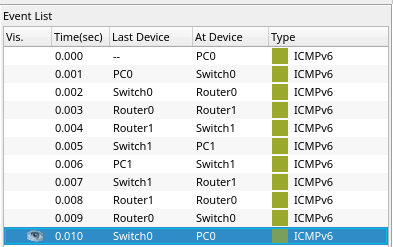
\includegraphics[width=0.7\textwidth]{imagenes/success.png}
    \caption{Ping PC0 a PC1}
  \end{figure}
\FloatBarrier
\section{Referencias}
Para la elaboración de este laboratorio se utilizó el siguiente material bibliografico.
\begin{itemize}
    \item \textbf{Video:} "GRE TUNNEL IPV6 TO IPV6 OVER IPV4 PACKET", Carlos Julio Peñaranda Herrera, 2022, at \url{https://www.youtube.com/watch?v=C7eEzr19aD0}.
    \item \textbf{Documento PDF:} "Configure IPv6 over IPv4 GRE Tunnel", Documentación de Cisco, 2019, at \url{https://www.cisco.com/c/en/us/td/docs/switches/lan/catalyst9500/software/release/17-9/configuration_guide/ip/b_179_ip_9500_cg/configuring_ipv6_over_ipv4_gre_tunnels.pdf}.
\end{itemize}

\end{document}
